% Findings prose as of Overleaf commit 1c3f21b (2026-09-05), moved out of main.tex
% when the section was reduced to a skeleton. Not \input anywhere. Salvage quotes,
% recording IDs and consent notes from here; do not restore the prose wholesale.

\section{Findings}
\label{sec:findings}
\subsection{empirical account of encounters at different sites}
Through our six sites, we found here are some empirical encountered patterns across each sites.

\textbf{Tappen Park (Staten Island)}Participants sometimes situated the robot against
the park’s local reputation, including concerns about drugs, public
safety, and how unfamiliar equipment might be treated there.
\textbf{Tappen Park (Staten Island)} Accounts there often drew on the existing distribution of trash receptacles and on
the presence of a mobile camera in a leisure setting. 
\textbf{Tappen Park (Staten Island)} The interview collected there explicitly connected the robot to the
surrounding Spanish-speaking, Latino, and Caribbean community
when discussing bilingual communication, culturally recognizable
design, and how the onboard camera might be interpreted.
\textbf{Tappen Park (Staten Island)} Unlike the park and street deployments,
this is a campus setting in which many users have an existing
relationship with the institution responsible for the space. Some
participants had seen TrashBot before or interpreted it in relation
to other technical projects and robots encountered on campus.
\subsection{The Shared Interpretation Process toward the encounter}
\label{sec:shared-move}
% Interpretation process, including what factors
% Similarity

The distinction between the street and park deployments and the two campus-based sites is especially relevant to institutional attribution. In a public park or commercial street, the organization behind an unfamiliar robot may not be apparent. At Cornell Tech or the Brooklyn Navy Yard, the setting itself gives participants more information about the organizations that might be responsible for a technical system. We retain this difference as part of the context in which participants' accounts were produced.

Before we come to what people said, it is worth establishing what they did,
because the two do not line up in the way a reader might expect.

At every site whose onboard footage we have reviewed, the dominant response to
the robot was not puzzlement but \emph{use}. People walked up to a machine they
had never seen before, whose provenance they could not have known, and put their
rubbish in it. The onboard record holds many such episodes, and they are notable
for how unremarkable they are: at Astoria Park a passerby walks directly to the robot,
drops waste in and leaves without breaking stride; at Tappen Park a man on a
bench holds out his drink can to the robot as it draws level with him, smiling
at it as he does (Figure~\ref{fig:everyday}a), and on another afternoon a man
finishes his drink after noticing the robot and puts the empty container in
because he wants to see what happens; in the Bronx a participant clears the
waste off their café table into it as it passes. A boy at Astoria Park, having
noticed the robot, searches his surroundings for something to throw
away---the machine's arrival creates the disposal rather than serving it.

\begin{figure}[t]
  \centering
  \begin{subfigure}[t]{0.49\columnwidth}
    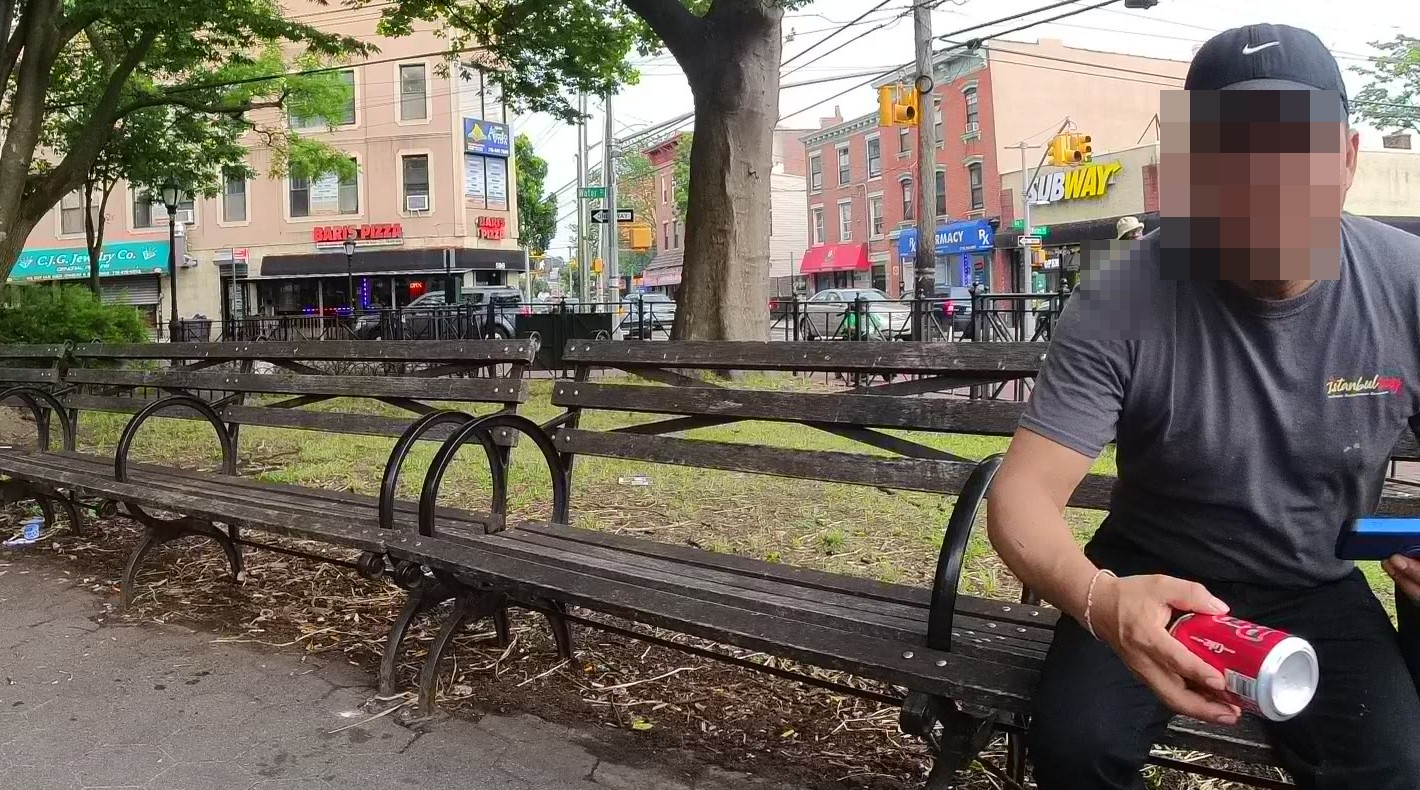
\includegraphics[width=\linewidth]{figures/vignettes/l_tappen_can.jpg}
    \caption{Tappen Park, 1 Jul}
  \end{subfigure}\hfill
  \begin{subfigure}[t]{0.49\columnwidth}
    \includegraphics[width=\linewidth]{figures/vignettes/m_astoria_phone.jpg}
    \caption{Astoria Park, 17 Jul}
  \end{subfigure}
  \caption{Two ordinary responses, from the robot's cameras (faces obscured).
  (a)~A man on a bench holds out his drink can to the robot as it draws level
  with him, from the forward-facing camera used in the first session.
  (b)~A participant raises his phone and films the robot as it approaches;
  the research team is on the bench behind him.}
  \Description{Left: from a low camera on the robot, a man in a cap and gray
  T-shirt sits on a long park bench and holds a red drink can out toward the
  camera, with shops and a pizzeria across the street behind him. Right: from
  the barrel's rim camera on a shaded park path, a man in shorts stands
  facing the camera holding a phone up in both hands; several people sit on a
  bench to the right. Faces are pixelated.}
  \label{fig:everyday}
\end{figure}

Three encounters are worth reading closely. Each was captured by the robot's
own camera (Figure~\ref{fig:vignettes}), and each shows the same recognition
doing different work: producing a request for permission, producing an object
to dispose of, and producing a refusal. We give the source recording and the
window in which each episode sits so that the material can be located in the
corpus.

\begin{figure*}[t]
  \centering
  \begin{subfigure}[t]{0.325\textwidth}
    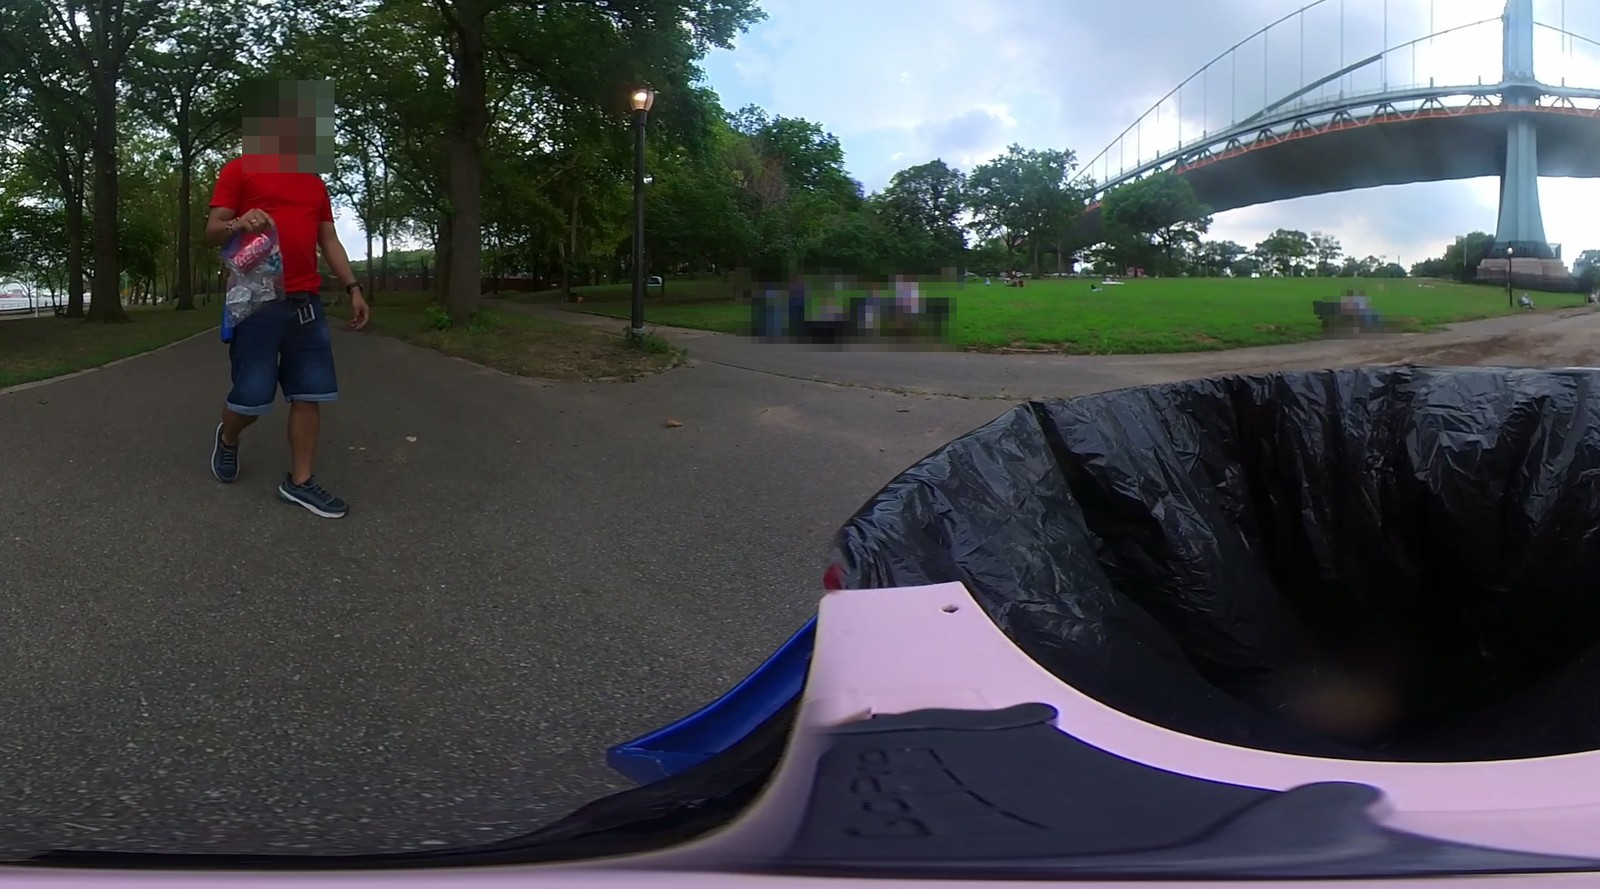
\includegraphics[width=\linewidth]{figures/vignettes/a_astoria_approach.jpg}
    \caption{Astoria Park, 15 Jul, 25:40}
  \end{subfigure}\hfill
  \begin{subfigure}[t]{0.325\textwidth}
    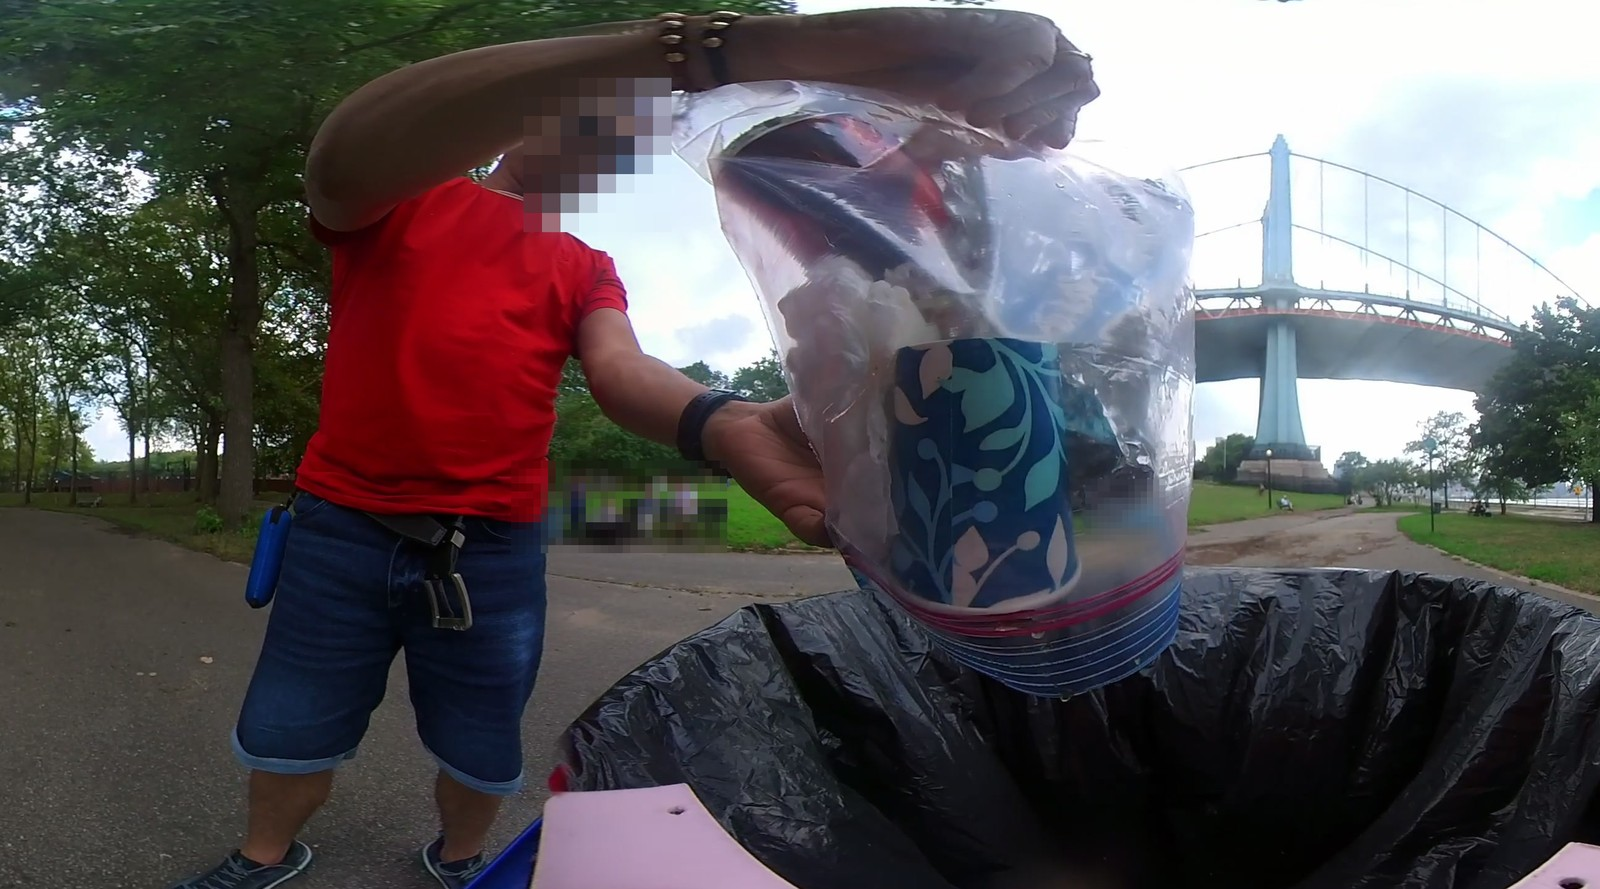
\includegraphics[width=\linewidth]{figures/vignettes/b_astoria_disposal.jpg}
    \caption{Astoria Park, 15 Jul, 25:43}
  \end{subfigure}\hfill
  \begin{subfigure}[t]{0.325\textwidth}
    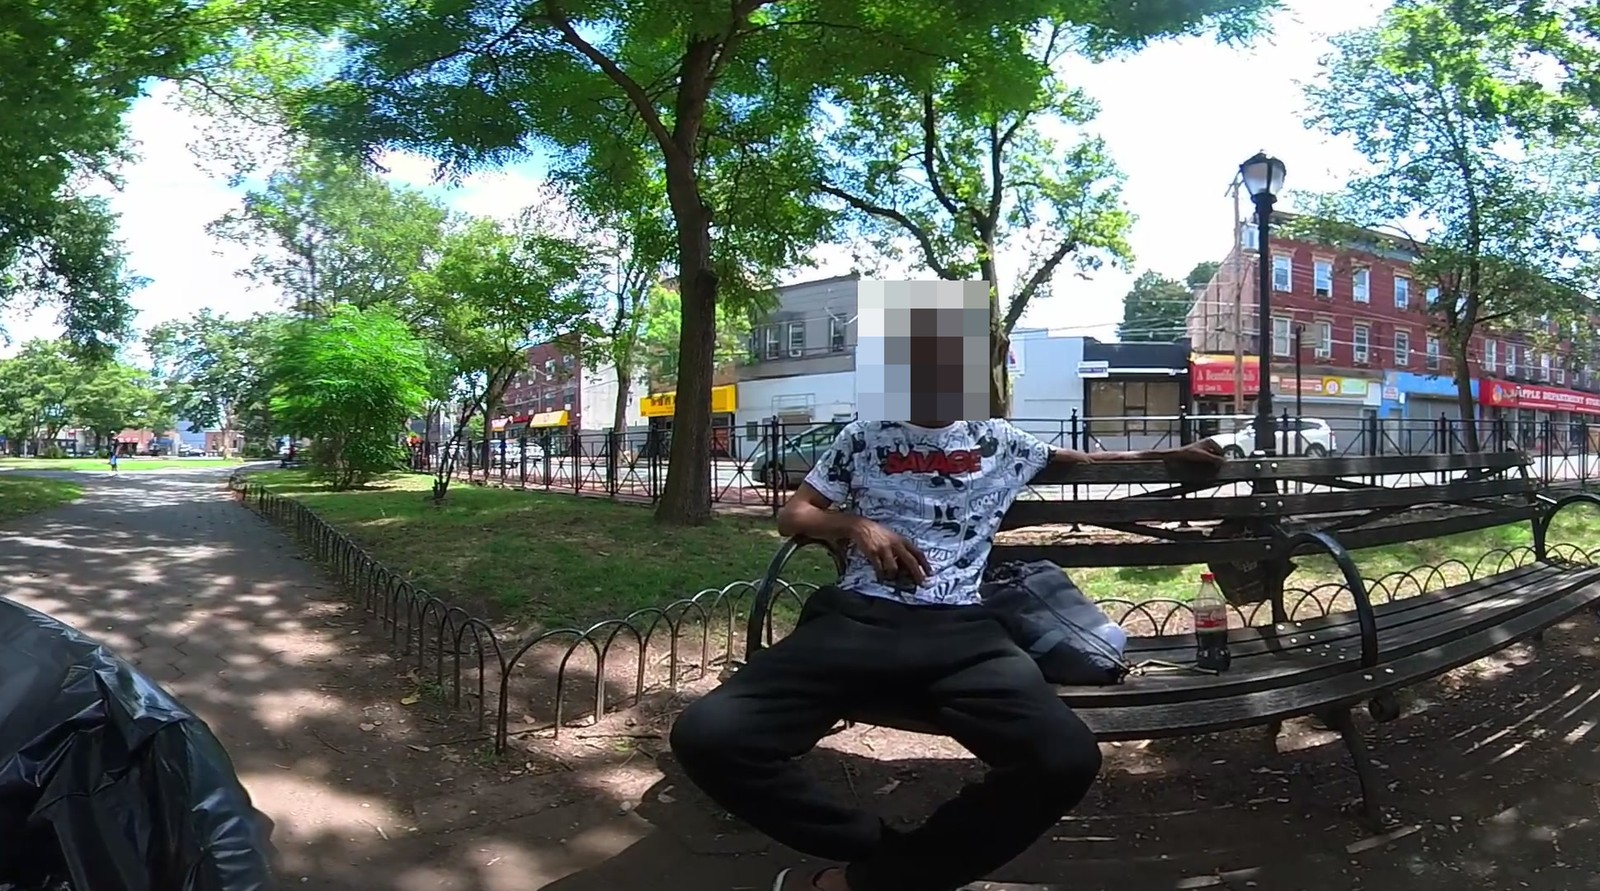
\includegraphics[width=\linewidth]{figures/vignettes/c_tappen_bench.jpg}
    \caption{Tappen Park, 7 Jul, 00:52 }
  \end{subfigure}\\[4pt]
  \begin{subfigure}[t]{0.325\textwidth}
    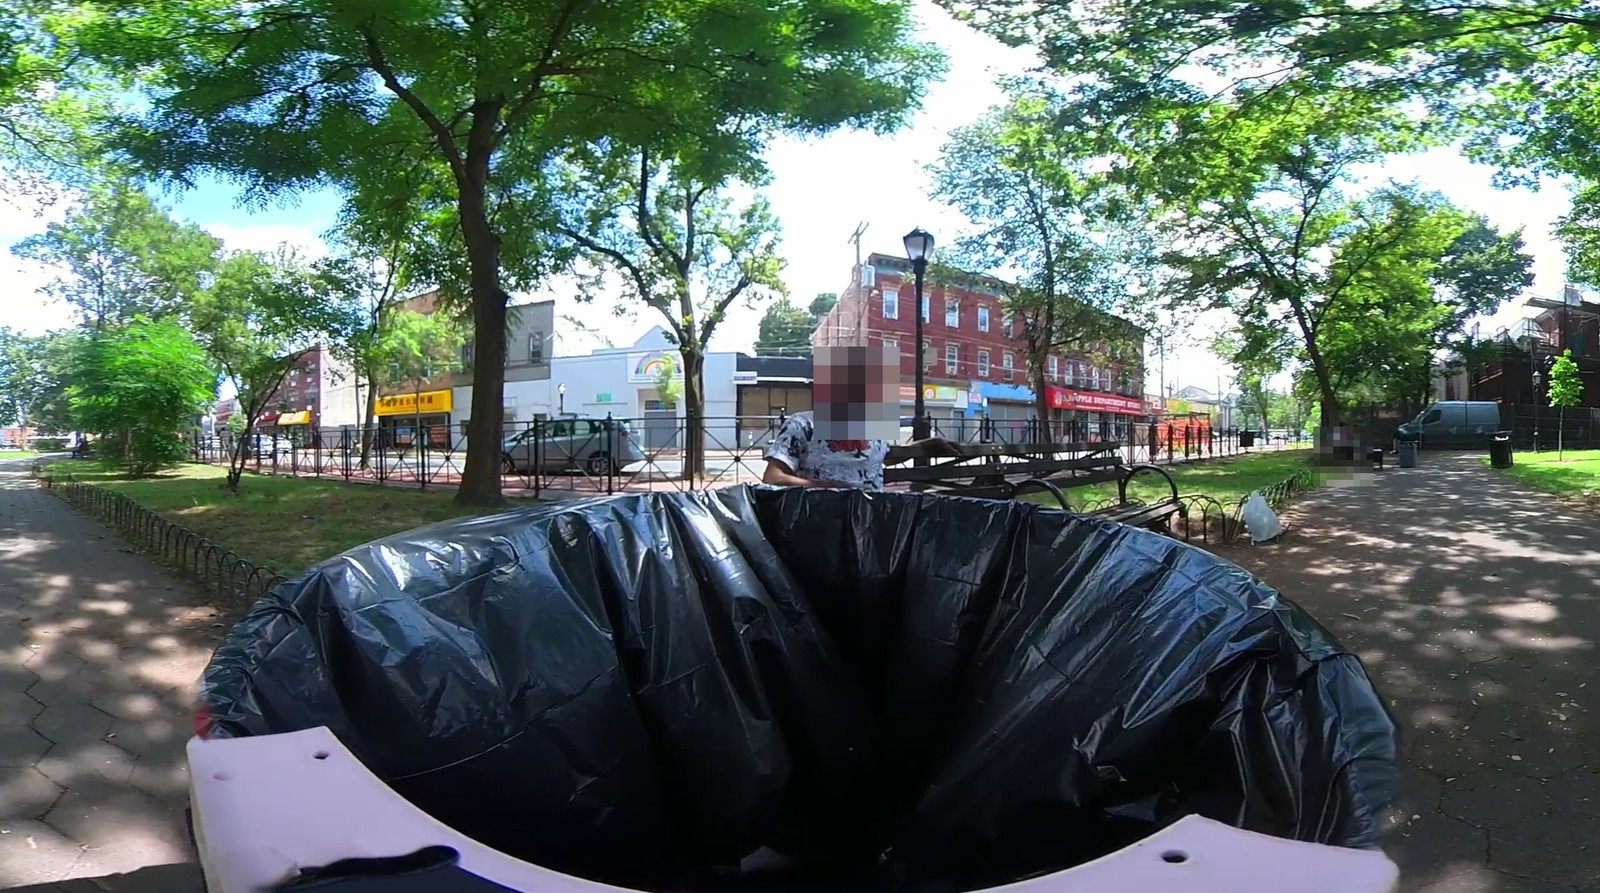
\includegraphics[width=\linewidth]{figures/vignettes/d_tappen_rim.jpg}
    \caption{Tappen Park, 7 Jul, 01:31 }
  \end{subfigure}\hfill
  \begin{subfigure}[t]{0.325\textwidth}
    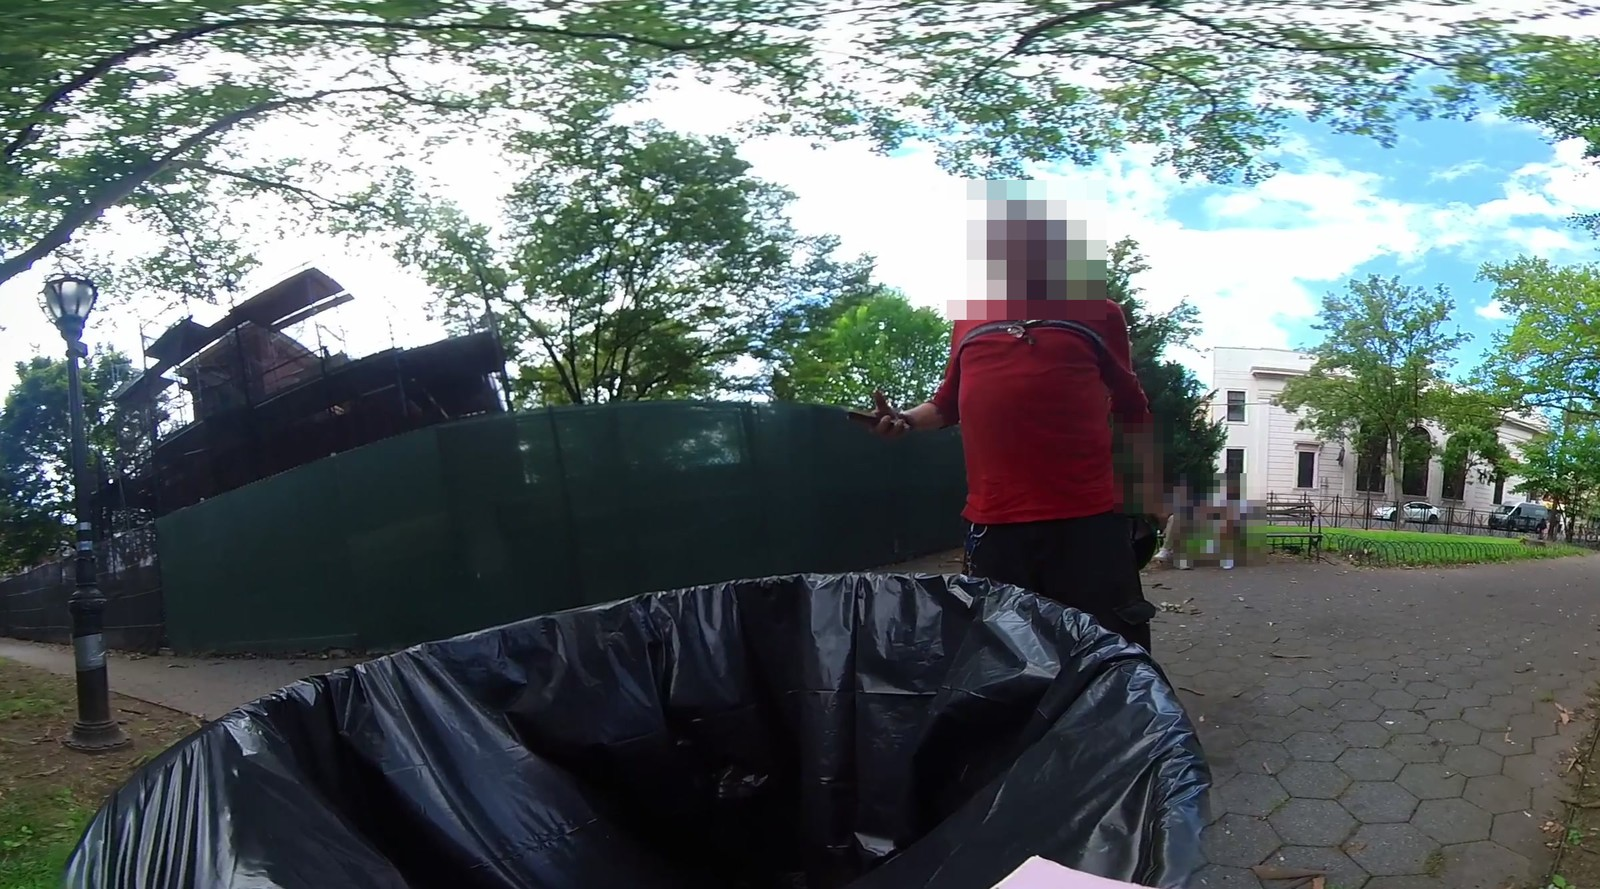
\includegraphics[width=\linewidth]{figures/vignettes/e_tappen_confront.jpg}
    \caption{Tappen Park, 7 Jul, 10:34 }
  \end{subfigure}\hfill
  \begin{subfigure}[t]{0.325\textwidth}
    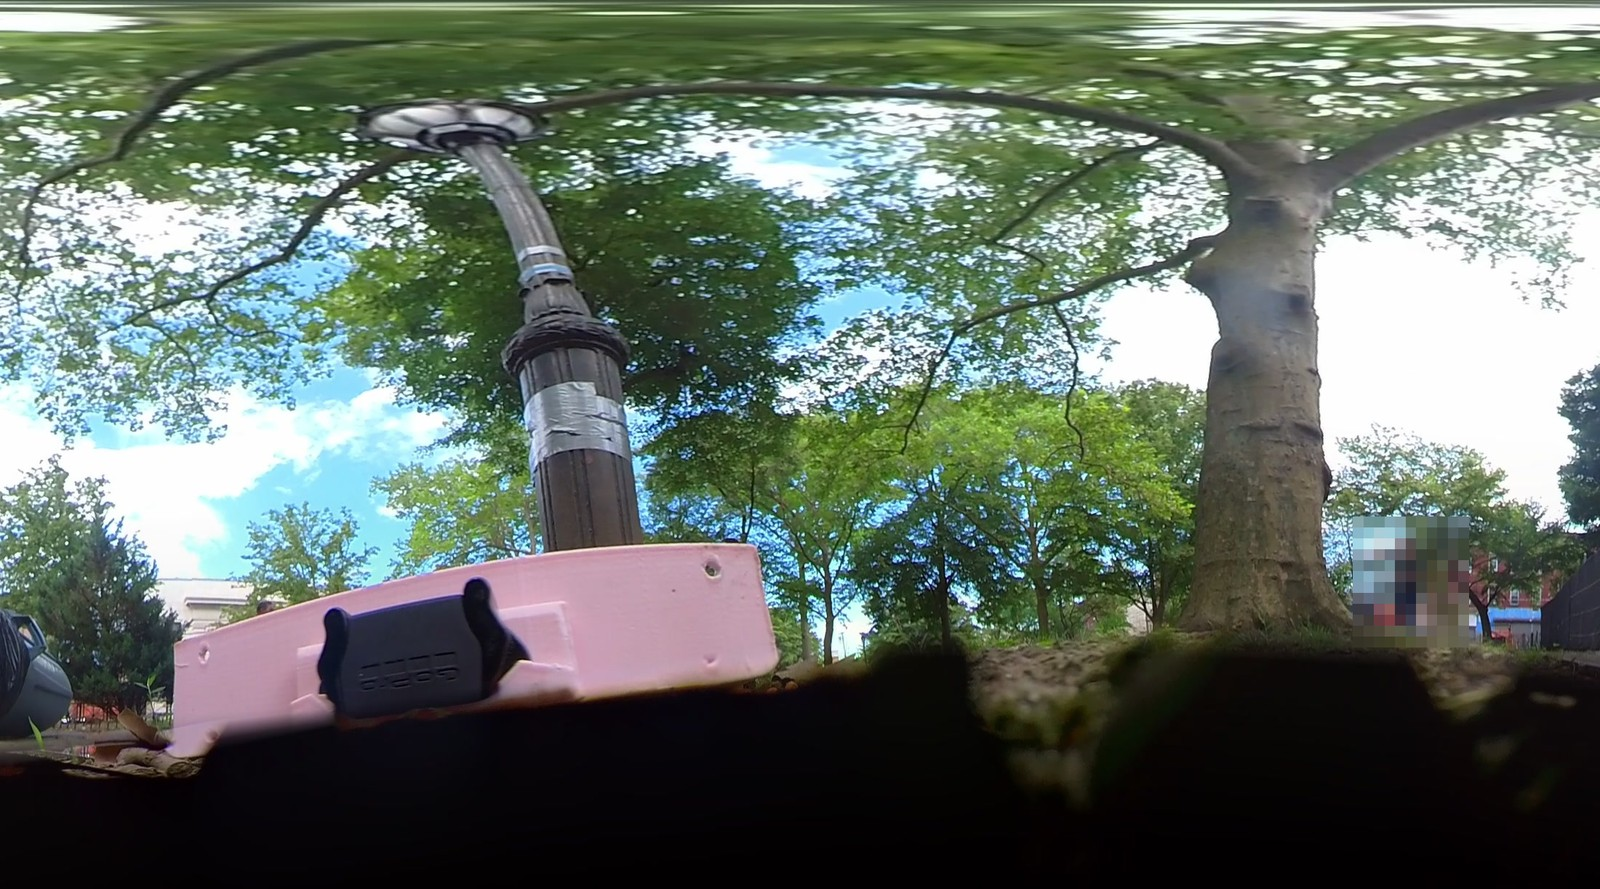
\includegraphics[width=\linewidth]{figures/vignettes/f_tappen_aftermath.jpg}
    \caption{Tappen Park, 7 Jul, 10:40 }
  \end{subfigure}
  \caption{The three encounters of \S\ref{sec:shared-move}, seen from the
  camera on the barrel's rim (faces obscured; times are within the session
  recording). (a)~The Astoria Park participant stops in front of the barrel
  with a sealed bag in hand; he has just asked the research team whether he is
  allowed to use it. (b)~Three seconds later the bag goes in---the one disposal
  in the corpus that the onboard camera records from an empty liner to the
  object at rest. (c)~At Tappen Park a man on a bench, a part-finished bottle
  of cola beside him, watches the barrel arrive. (d)~Forty seconds later he
  reaches across the rim as the barrel turns toward him; the bottle, clear
  plastic against a black liner, is not resolvable in the frame.
  (e)~The same afternoon, another participant stands over the barrel and
  addresses its camera directly (\pquote{you're staring at me with a camera
  like this}). (f)~Six seconds later, after he has knocked the barrel over:
  the camera now lies on the ground beside its own rim.}
  \Description{Six photographs taken by the 360-degree camera mounted on the
  rim of the trash barrel robot, so the black liner and pink rim appear in the
  foreground of each. Top row: on a park path with a suspension bridge behind,
  a man in a red shirt walks toward the barrel holding a clear bag, then holds
  the bag over the liner as a printed cup slides out of it; on a curved park
  bench a man in a white printed T-shirt sits with a cola bottle beside him,
  looking at the camera. Bottom row: the same man stands behind the rim with
  his hand at its edge; in a paved park square with a green construction
  fence, a man in a red shirt stands over the barrel gesturing at the camera;
  in the last frame the view is tilted onto the ground, with the pink rim
  lying on the paving and a tree and lamppost rising above it. All faces are
  pixelated.}
  \label{fig:vignettes}
\end{figure*}

\paragraph{Asking a trash can for permission.}
At Astoria Park on 15 July the robot's onboard camera shows the inside of its own
liner empty for the first twenty-five minutes of the recording
(\texttt{VID\_20250616\_\allowbreak 054414\_\allowbreak 00\_011};
Figure~\ref{fig:vignettes}a--b). At 25:38 a man stops squarely in front
of the barrel and holds a sealed transparent bag in front of him for roughly two
seconds before anything else happens; at 25:42 a hand carrying a printed
cylindrical container crosses the rim, color appears against the black liner, and
the object remains there through the end of that recording and into the next.
This is the only disposal in our corpus that the robot's own camera documents end
to end, from an empty liner through the act to the object at rest.

What makes it worth the space is the pause. Before disposing, he asked the
research team whether he was allowed to. The recruitment turn on the interview
recording opens by noting that a family member ``has interacted with our robot,''
and the researcher later asks, through the interpreter, why he ``asked us the
permission to dump trash to it.'' The answer relayed back is that the machine
looked to him like something still being built---a prototype in a study---and
that he was unsure it was able to accept rubbish yet. He read the barrel
correctly as a receptacle and simultaneously as an object under construction, and
it is the second reading that produced the request. Nothing about the form of a
trash can asks to be asked; the visible research apparatus around it does.

We can report this participant's conduct with confidence and his account only at
a remove. He spoke Spanish and was interviewed through a relative, and, as
\S\ref{sec:limitations} sets out, our transcription pipeline rendered his speech
as approximate English rather than flagging it as unhandled. The conduct is the
part of this case the record holds firmly, which is precisely why we lead with
it.

\paragraph{Making the trash in order to use the machine.}
At Tappen Park a man noticed the robot, looked around for something to put in it,
found nothing, finished the drink he was holding, and disposed of the empty
bottle. Both parties describe the sequence on the same recording. He gives the
order of operations himself---\pquote{everything there is trash, and that's my
present, so \ldots I've looked around to see if there was trash there}---and the
researcher, recruiting him afterwards, names what she had watched him do:
\pquote{I noticed that you actually had your bottle of coke, it still had
something, but then you finished it, so you could throw it inside.} His stated
reason is not disposal but trial: \pquote{it's like a new experience, like I
really want to \ldots try with this.}

The obvious alternative reading---that he had rubbish and the robot was
convenient---is closed off by the participant himself. He had no rubbish. He made
some. The machine did not serve a disposal need, it produced one, and the account
he gives of why is about wanting to find out what the thing would do. The
recycling barrel's own camera holds the outline of the sequence
(\texttt{VID\_20250608\_051940\_00\_001}; Figure~\ref{fig:vignettes}c--d): at
00:52 he is on the bench with the bottle beside him, part of the drink still in
it, and at 01:31, as the barrel turns toward him, he reaches across its rim.
What the camera cannot resolve is the object: a clear bottle against a black
liner leaves no trace in the frame, so the account, given by both parties on
the same recording, remains the record of what went in.

\paragraph{``It turned from cute to offensive.''}
The same afternoon produced the sharpest refusal in the corpus, and it is on the
robot's own recording (\texttt{VID\_20250608\_054047\_00\_003}, 09:30--12:00;
Figure~\ref{fig:vignettes}e--f). A man addresses the barrel directly, at first
playfully---he names it R2D2 and threatens to send it after a companion---and
then, as it holds its position near him, with an objection to the camera:
\pquote{don't video us \ldots you're staring at me with a camera like this}.
He knocks it over. From the ground the camera keeps looking, and the objection
continues at it---\pquote{take it somewhere else}, \pquote{don't ever come in my
face and look at me}, \pquote{I don't like my picture}---for most of a minute.

What follows is the part that matters. He apologizes---not to the researchers, to
the machine: \pquote{I'm sorry, buddy \ldots I didn't mean to hurt you. I didn't
mean to make you cry.} In the interview minutes later he states the objection in
terms that are about the place rather than the device---\pquote{everything is
under the eye of the sky these days, and it takes away a sense of
freedom}---and then asks the robot, rather than the interviewer, to carry the
complaint back: \pquote{can you please note that in your memory}, and again,
\pquote{please keep that in your net}. His own summary of the arc is the cleanest
statement of it available to us: \pquote{that's why it turned from cute to
offensive}.

Read against \S\ref{sec:probe}, this encounter does everything a probe is
supposed to do. The barrel is legible enough to be named, addressed, apologized
to, and enlisted as a channel to whoever is behind it, and illegible enough that
the question of who is watching through it stays open long enough to harden into
an objection. Tipping a robot over is usually reported either as vandalism or as
evidence of diffuse hostility to
automation~\cite{brscic2015escaping,salvini2010safe,nomura2016why}. Here it is
neither: it is the middle of a sequence that opens with a \emph{Star Wars}
reference and closes with an apology, and what it registers is a specific
objection to being recorded in a specific park.
% \todo{AUDIO VERIFICATION: the quoted lines in the three vignettes above come from
% our working transcripts and still need to be checked against the source audio
% before camera-ready, per \S\ref{sec:interview-analysis}. Files:
% \texttt{TP-P09-conduct}, \texttt{TP-P09-interview},
% \texttt{IMG\_7447} (TP-P11). The Astoria Park case (\texttt{IMG\_1745}) is
% deliberately reported without verbatim quotation from the participant.
% Timeline of the Tappen Park refusal re-checked 2026-09-02 against the onboard
% frames and a fresh large-v3 pass over 09:00--12:00 of \texttt{\_003}: the
% barrel goes over at about 10:35, during the ``you're staring at me'' turn;
% ``take it somewhere else'', ``don't ever come in my face'' and ``I don't like
% my picture'' all come after it, from the ground; the apology runs 11:32--12:00.
% The old cut's line ``I will not put any other'' ($\approx$11:24) reads as
% ``we're not performing anything'' on the new pass, so it is no longer quoted as
% a refusal to use the bin; restore it only if the audio confirms it.}

This recognition does not appear to require a shared language, and two Astoria
Park encounters make the point by separating the two things. The first is the
case just described: the participant used the robot without hesitation, and it
was only the conversation afterwards that had to be routed through a relative,
whose summary was that it would be good to see such robots throughout the
community. In the second, researchers and
participants spent the opening of the interview negotiating how to communicate at
all, trying and failing to find translation software between them; the
participants had nonetheless been sitting beside the robot's route watching it
work. In neither case was using or understanding the machine the difficulty.
Talking about it afterwards was. Nor does it
require prior familiarity with robots, or any resolution of the question of who
sent the machine. The form does the work: a barrel-shaped container with an open
top, arriving where you are.

Most importantly, recognition and use do not require approval. This is the
finding that sets up everything after it. The Bronx participant who cleared their
table into the robot spent the subsequent interview arguing that it did not
belong on that block---that it would obstruct pedestrians, that it would not
survive the winter, that it was better suited to an enclosed space. An Astoria
Park participant who watched the robot with visible curiosity screamed and
retreated each time it came near, then gave a considered interview about how a
friendly trash identity would be more acceptable than a policing one. Use and
endorsement come apart routinely.

There are limits to what this shows, and they are specific enough to state
plainly. Our behavioral record is uneven in two distinct ways. Coverage is uneven
\emph{across} sites: onboard footage has been reviewed for the Staten Island,
Queens and Bronx sessions but not yet for Manhattan or Brooklyn, so ``at every
site'' in this subsection means every site whose conduct we have been able to
look at. Readability is uneven \emph{within} sessions, because the onboard camera
sits at the barrel's rim and sees the inner wall of the liner rather than its
floor. The rim is in frame for only part of each recording---in the sessions we
measured, for roughly a quarter of one Little Italy session and for almost none
of the Starlight Park material---and low-contrast items such as clear plastic or
thin brown sticks leave no visible trace against a black liner even when the rim
is in view. We therefore treat an absence of visible disposal as uninformative
rather than as evidence of non-use, and we do not report disposal rates or
compare them across sites. What we can say is that across three structurally
unalike settings---a riverside park, a neighborhood park with a difficult
reputation, and a dense commercial corridor---the machine was read as a
receptacle and used as one, quickly, by people who went on to disagree profoundly
about whether it should be there.

Which poses the puzzle this paper is about. If everyone recognizes the robot in
the same way and uses it in the same way, why do the accounts they give of it
differ so sharply from place to place?

\subsection{The Local Inputs: how encountered sites play in the interpretation}
\label{sec:inputs}

The answer is that the accounts are not different \emph{questions}. Participants
everywhere asked the same small set: who runs this, what will happen to it, what
is it seeing, and is it needed here. What differed was the material each place
made available for answering them. We organize this section by the resource
recruited rather than by borough, because a section per site would reintroduce
the claim we are arguing against---that place is a variable acting on people
rather than a supply of things to think with. Figure~\ref{fig:arthur} shows
three of those things in the robot's own field of view on a single Bronx
block: a caf\'e table, a municipal litter basket with the person paid to work
it, and a man who had already decided what the neighborhood would do to an
unattended machine.

\begin{figure*}[t]
  \centering
  \begin{subfigure}[t]{0.325\textwidth}
    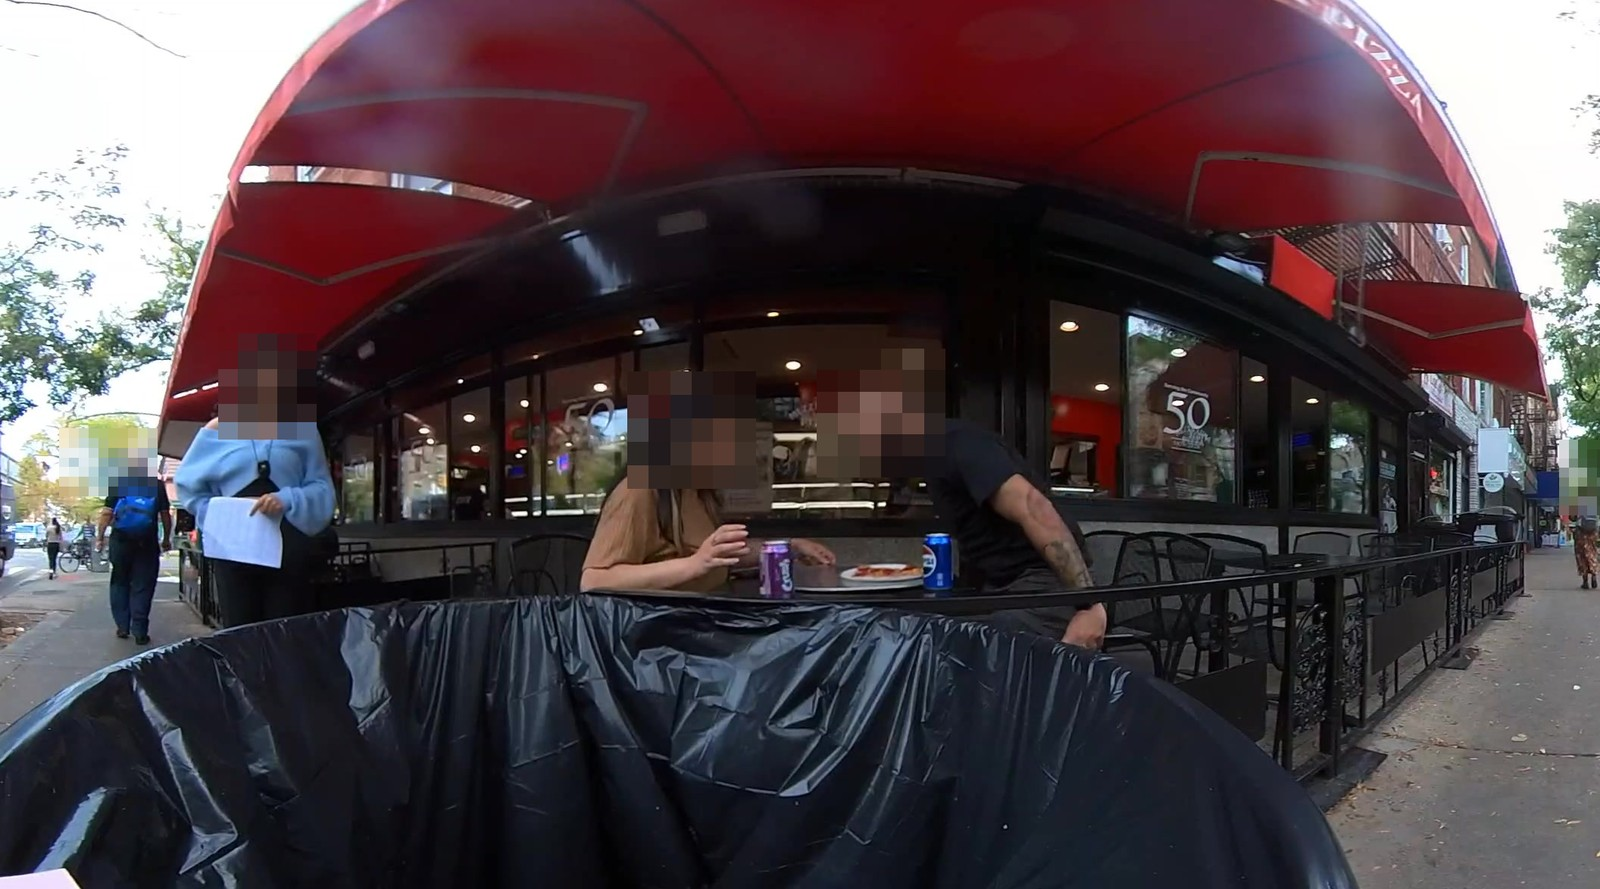
\includegraphics[width=\linewidth]{figures/vignettes/i_arthur_table.jpg}
    \caption{22:35}
  \end{subfigure}\hfill
  \begin{subfigure}[t]{0.325\textwidth}
    \includegraphics[width=\linewidth]{figures/vignettes/j_arthur_sanitation.jpg}
    \caption{25:45}
  \end{subfigure}\hfill
  \begin{subfigure}[t]{0.325\textwidth}
    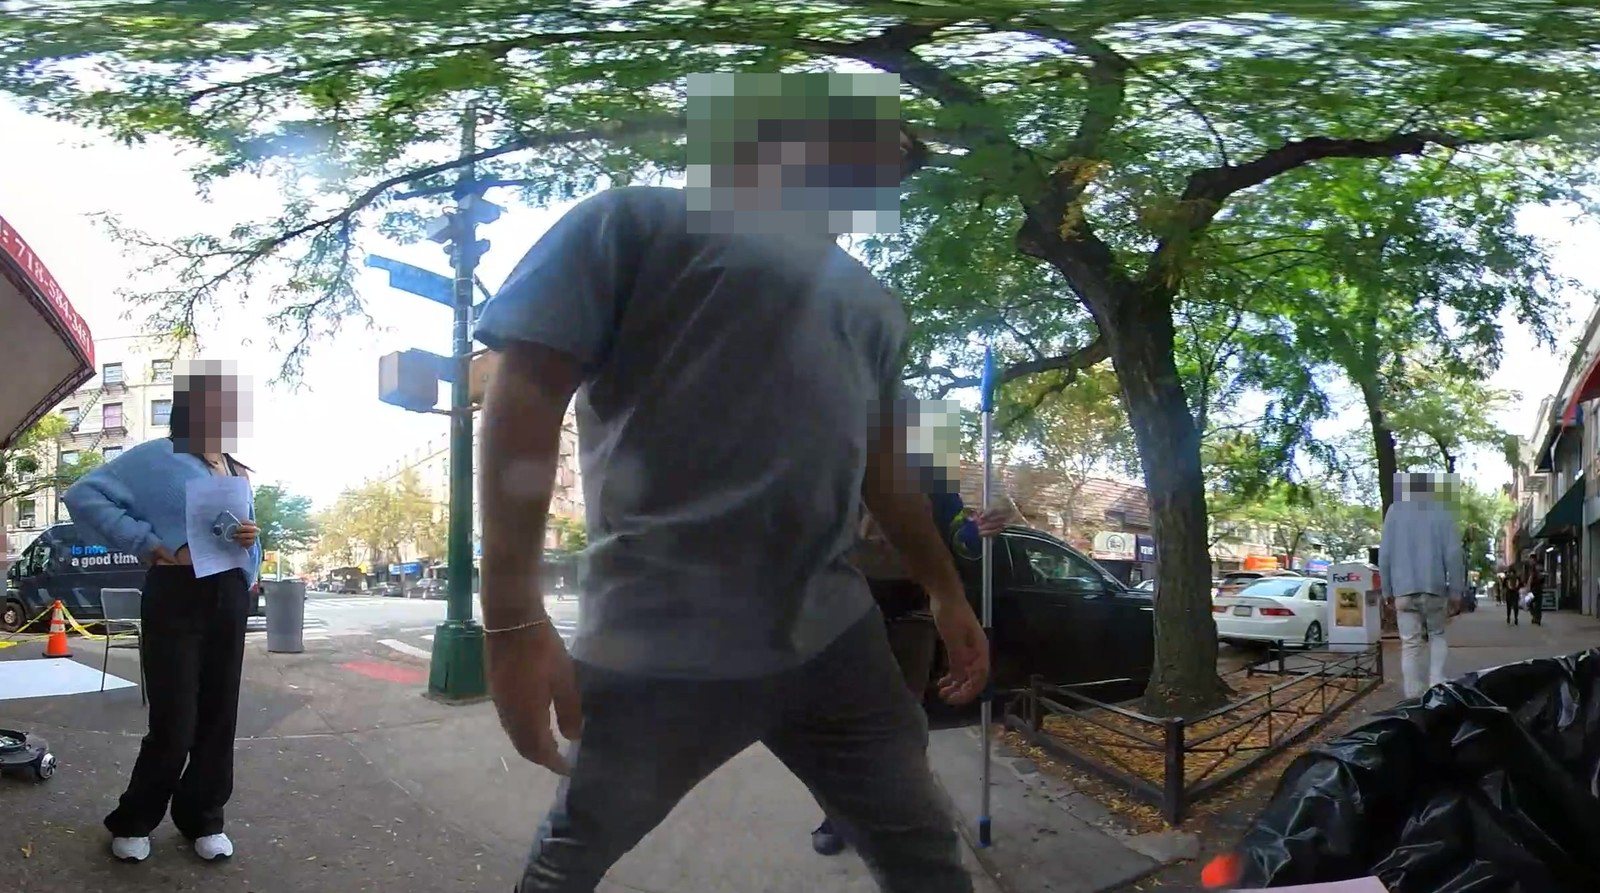
\includegraphics[width=\linewidth]{figures/vignettes/k_arthur_vendor.jpg}
    \caption{28:36}
  \end{subfigure}
  \caption{One block, three resources: Arthur Avenue, 29 September, from the
  camera on the barrel's rim (faces obscured; times within the session
  recording). (a)~The robot stops at a pizzeria's sidewalk table and the two
  people eating there reach across its rim in turn---the participant whose
  interview then explained that it did not belong on the block
  (\S\ref{sec:said-did}). (b)~Three minutes later it stands beside a municipal
  litter basket while a public-safety officer on sanitation duty looks it
  over: the labor the block's residents measured it against. (c)~The
  participant who told us that \pquote{anything is not tied down over here}
  inspects it after being called across the sidewalk.}
  \Description{Three photographs from the trash barrel robot's rim camera on
  a commercial street. Left: under a red pizzeria awning, a woman and a man
  sit at a sidewalk table with a plate and drink cans while the man leans
  toward the barrel's black liner in the foreground; a researcher with a
  clipboard stands behind them. Middle: a man in a yellow high-visibility
  vest marked SANITATION stands with his back to the camera beside a blue
  municipal bin and a wire litter basket, with a street sign, caution tape and
  a delivery van behind. Right: a man in a gray T-shirt stands over the
  barrel looking down at it, with a tree-lined sidewalk and parked cars
  behind. All faces are pixelated.}
  \label{fig:arthur}
\end{figure*}

\paragraph{Institutional reading: who runs this?}
The most consequential thing a participant can decide about a public robot is
whose it is, and the candidate owners are supplied entirely by the setting. At
Starlight Park, in a neighborhood the participant described as heavily
Spanish-speaking and predominantly Latino and Caribbean, the question arrived
already answered: \pquote{in this neighborhood, I feel like a camera is going to
make folks feel like, who's watching? You know? Is this the police, you know?
\ldots Or even, is this ICE?} The camera raises a general question; the
neighborhood supplies the specific list. On Arthur Avenue a participant went
straight to jurisdiction rather than technology, asking where we thought we would
be permitted to operate and observing that street cleaning there is already tied
to the sanitation department and to the business associations that clean the
block. At Astoria Park the same question resolved benignly---one participant
assumed the machine was the city's and was reassured by that, while another
distinguished a university experiment from what a municipal version of the same
device would mean, and a third read it directly as robotic policing and worried
about automated authority. Same question, four different answers, each drawn from
what the asker knew about who operates things where they live.

\paragraph{Threat reading: what will happen to it?}
Where a neighborhood has a reputation, participants applied it to the robot's
survival rather than to their own safety. In the Bronx this produced the most
consistent set of accounts in the corpus: the robot would be stripped for parts
almost immediately, and the parts would be sold. One participant was explicit
about both the mechanism and the reason---\pquote{they will take anything to make
money to buy drugs}---and concluded not that the design should be hardened but
that it should be retrieved: \pquote{Here, no way. No way. You got to bring it
inside with the remote control.} Another located the risk in the community he
claimed as his own, in the sharpest formulation we recorded:
\pquote{Anything is not tied down over here} (Figure~\ref{fig:arthur}c) and \pquote{People who steal here is
the ones who live here}, with the prediction that \pquote{Eventually it'll work
here once the crime rate goes away}. At Tappen Park the same reading attached to
a specific local history of drug activity in the park, and produced a
correspondingly specific design recommendation: operate in daylight only. Note
what is not happening here. These participants were not describing a fear of the
robot. They were describing a place, and the robot was the thing that place would
act upon.

The clearest evidence that this reading is supplied rather than carried is its
absence. At the Brooklyn Navy Yard---an access-controlled industrial campus where
the people we spoke to were there to work---not one of the eight participants
raised theft, stripping, vandalism or tampering, unprompted or otherwise. The
same robot, presented the same way, in a place that offers no story about what
happens to unattended property, simply did not occasion the question. If a
disposition toward robots travelled with people, we would expect the theft
reading to appear at some rate everywhere. It appears where the place supplies
it.

\paragraph{Bodily and privacy reading: what is it seeing?}
What a camera means depends on what the place is used for. Astoria Park's lawns
are where people sunbathe, and the privacy concern there was about bodies:
\pquote{\ldots people with bikini \ldots don't want to be filmed.} One
participant, smoking when the robot approached, moved away from it and afterwards
asked that the camera be made clearly visible and the robot keep about five feet
back; another set the boundary at six feet and grounded it in hygiene rather than
surveillance. For others in the same park the camera was an invitation to film
back: two participants raised their phones and recorded the robot as it came
toward them (Figure~\ref{fig:everyday}b). On the Bronx sidewalk the same
question produced a boundary rather
than a distance, drawn at the threshold of the home---a participant held that
such devices should not invade privacy while observing \pquote{But you ain't in
your house, you're on the streets}, which left the street camera unobjectionable.
At the Roosevelt Island café the reading shifted again, and in a way that follows
from the setting: participants there reasoned about recording as a matter of
procedure and consent rather than of watchers, noting that a machine moving
through a space where people have not consented to being filmed is a problem
about permission, and that audio and video collection ought to be consented to.
That is a campus population applying a campus norm, and it recurs at the Navy
Yard, where a participant made consent the whole of the test---recording was
fine as we were doing it, but \pquote{if it's like, you know, unconsentially,
that's a bit, like, weird}, which he glossed as \pquote{major privacy}.

The Navy Yard also produced two readings of the camera that are not about
watching at all. One participant treated it as constitutive of the machine rather
than as an addition to it, and so as not raising a question: asked whether the
camera changed how he felt, he replied that it did not, because
\pquote{the camera is because it's robot, right? It cannot be without camera,
right?} Another reframed it as an instrument for measuring a public problem,
approving of the recording precisely because it would show how much rubbish is
actually being thrown away here. Both are available only to
someone who has already settled the question of who is operating the thing, which
on a campus one is employed at is a question that mostly settles itself.
\note{Quote policy for Brooklyn: only NY-P02 and NY-P04 have an explicit
recording request captured on tape, so only those two are quoted verbatim here.
NY-P05's camera-as-measurement line is paraphrased for the same reason and should
be promoted to a quote if the consent record turns out to be complete. See
\texttt{transcripts/Brooklyn-NavyYard/\_NY-P\_index.md}. NY-P01 is quarantined
pending review --- he said he did not want himself recorded, on video or audio,
and no consent request appears in that recording.}

\paragraph{Infrastructural-fit reading: is it needed here?}
The most common evaluation was not about the machine at all but about whether the
work it does is already being done. This is where the same interpretive move most
visibly produces opposite conclusions. On Arthur Avenue a participant explained
that his block would not benefit, because \pquote{the community already have
their porters that clean here every single day}, and then performed the
allocation himself, redirecting the robot to 125th Street, 149th and Kingsbridge
on the grounds that those streets are genuinely dirty. A merchant on the same
block reached the same verdict by a different route---landlords already handle
the bins building by building, so the robot was \pquote{useless}---and a group of
students objected that \pquote{there's three trash cans on the street}. That
labor was in the frame as well as in the accounts: the robot's own camera
caught it stopped beside a municipal litter basket while a public-safety
officer on sanitation duty looked it over (Figure~\ref{fig:arthur}b). At
Astoria Park, where receptacles are sparse relative to footfall, the identical
reasoning ran the other way: there are no bins here, so the robot is useful, and
useful specifically on crowded weekends. The robot did not change. What changed
was the sanitation infrastructure it was being measured against.

Within this reading sits the corpus's only first-person account of the labor in
question. A sanitation worker interviewed on her own route moved, within a single
turn, from displacement anxiety---\pquote{My only, like, question is, does that
have an effect over what I do?}---through a favorable assessment
(\pquote{It looks like it makes people job, my job easier}) to the institutional
form of the worry: that her employer, not the machine, would draw the conclusion
that \pquote{we won't need that many workers}. Her camera concerns dissolved
against a neighborhood she described as already saturated with recording. No
other participant had access to this resource, because no other participant does
this work here.

\paragraph{}
Across all four families the structure is the same. The question is general and
recurs everywhere; the answer is assembled from what the place puts in reach; and
because the places differ in what they put in reach, the same interpretive
practice yields conclusions that look, from the outside, like different attitudes
toward robots. They are not. They are one practice, locally supplied.
\note{Quote provenance: the Bronx and Starlight lines are transcribed verbatim
with timestamps in the Bronx analysis deck; the Astoria bikini line and the
Tappen daylight line are audio-verified; the remaining Queens and Tappen material
is analyst paraphrase from the site decks and is deliberately rendered as
reported speech here rather than quoted. Verify the sanitation-worker lines
against audio before camera-ready --- ASR renders ``we won't need that many
workers'' as ``we won't meet that much workers''.}

\subsection{The Said--Did Relationship}
\label{sec:said-did}

\S\ref{sec:shared-move} established that people use the robot without endorsing
it, and \S\ref{sec:inputs} that their endorsements are assembled from local
material. The paired cases---encounters for which we hold both the robot's
record of what a participant did and that participant's later account of
it---let us watch those two facts meet in a single person. This section is
deliberately narrow. It reports the cases we can state with confidence, it does
not count them, and it draws one conclusion from them: that account and conduct
are produced at different moments, under different demands, and that what moves
the account is not information about the machine but the standing of a single
question, who is behind it. Table~\ref{tab:paired} lists the cases and the
record that supports each side of them.

Across these cases we distinguish four relationships between what a participant
did and what they went on to say. In \emph{convergence} the account matches the
conduct; in \emph{divergence} it does not; in \emph{elaboration} the account
supplies reasoning the conduct could not have revealed; and in \emph{trajectory}
the relationship shifts within the encounter itself. These describe cases rather
than sort participants, and they do not carry equal weight. If attitudes were
stable dispositions, conduct would express them; if accounts are assembled in
the moment, they may still land where the conduct did. Convergence and
elaboration are therefore compatible with the account we are proposing and with
the one we are arguing against. The evidential weight sits on divergence and
trajectory.

\begin{table*}[t]
  \caption{Encounter-plus-account cases discussed in \S\ref{sec:said-did}, with
  the record that supports each side. Dates are session dates; onboard windows
  are given by time within the session recording.}
  \label{tab:paired}
  \small
  \setlength{\tabcolsep}{5pt}
  \begin{tabular}{@{}>{\raggedright\arraybackslash}p{0.15\textwidth}>{\raggedright\arraybackslash}p{0.33\textwidth}>{\raggedright\arraybackslash}p{0.30\textwidth}>{\raggedright\arraybackslash}p{0.16\textwidth}@{}}
    \toprule
    Case & Did & Said & Relationship \\
    \midrule
    Astoria Park, 15 Jul & Paused with a bag in hand, asked the team for permission, disposed (rim camera, 25:38--25:44) & The machine looked like a prototype not yet able to take rubbish (interview, via interpreter) & Convergence; elaboration \\
    Tappen Park, 7 Jul, trial & Looked for rubbish, found none, finished his drink, reached across the rim (onboard, 00:52--01:32, Fig.~\ref{fig:vignettes}c--d; disposal witnessed by researcher) & \pquote{a new experience \ldots I really want to try} (interview, both voices) & Elaboration \\
    Tappen Park, 7 Jul, refusal & Named it, objected to its camera, knocked it over, kept objecting, apologized to it (onboard, 09:30--12:00; Fig.~\ref{fig:vignettes}e--f) & \pquote{under the eye of the sky}; asked the robot to remember the complaint (interview) & Convergence; trajectory \\
    Arthur Avenue, 29 Sep & Reached across the rim as the robot stopped at his caf\'e table (onboard, 22:33--22:36, Fig.~\ref{fig:arthur}a; interview opening) & Does not belong on this block: foot traffic, winter, better indoors (interview) & Divergence, use~$\rightarrow$~objection \\
    Astoria Park, 16 Jul & Screamed and moved away at each approach, kept watching from a distance (onboard, 14:44--15:13; Fig.~\ref{fig:retreat}) & Theft, surveillance, the police robot dogs; \pquote{at least it's kind of friendly} (interview) & Divergence, avoidance~$\rightarrow$~appraisal \\
    Little Italy, 29 Sep & Came over alarmed at the camera (interview; onboard not located) & Alarm, then a game, on learning that a person was driving it (interview) & Trajectory, produced by disclosure \\
    Tappen Park, 7 Jul, operator & Watched, let it approach (interview; onboard not located) & \pquote{I thought you guys directed it to me \ldots so I wasn't scared} (interview) & Trajectory, self-produced \\
    \bottomrule
  \end{tabular}
\end{table*}

\paragraph{Convergence.}
The refusal at Tappen Park (\S\ref{sec:shared-move}) is the clearest convergent
case in the corpus, and it is instructive because it is unsurprising. The
objection the man states to the barrel as it holds position beside
him---\pquote{you're staring at me with a camera like this}---is the objection
he restates to an interviewer minutes later, now attached to the place rather
than the device: \pquote{everything is under the eye of the sky these days}.
Conduct and account line up, and they line up because both were assembled from
the same local material, a camera in a park with a reputation, read as watching.
The Astoria Park participant who asked permission before disposing is convergent
in the same sense: a visibly careful approach, and an account of the machine as
something still under construction. What convergence cannot tell us is whether
the account expressed a disposition the conduct had already enacted, or was
produced afterwards and happened to land where the conduct did. Both readings
fit, which is why we do not build on these cases.

\paragraph{Elaboration.}
Two cases show the interview doing work the footage cannot. The pause on the
Astoria Park recording is, on video, two seconds of a man holding a bag; the
interview supplies what filled them, a reading of the research apparatus around
the barrel as a sign that the thing was not finished. The Tappen Park trial is
the same relation run the other way: the footage shows a man on a bench and,
forty seconds later, a hand across the rim, but the account gives the order of
operations---look for rubbish, find none, finish the drink---that turns an
ordinary act of disposal into an experiment the participant ran on the
machine. Elaboration tells us something about interview
method: it is where the local resources of \S\ref{sec:inputs} become visible,
because they are named rather than enacted. It does not by itself tell us where
those resources were when the conduct happened.

\paragraph{Divergence, in both directions.}
Divergence is the case that separates the two accounts, and we have one instance
in each direction. A participant on Arthur Avenue used the robot as it arrived at
his caf\'e table, and then spent the interview explaining that the machine did
not belong on that block: too much foot traffic, no good in the snow, better
suited to somewhere enclosed. Two records establish the disposal. The interview
opens with the researcher thanking him for using the bin and with his accepting
the thanks without correction, and the onboard recording places the robot at
the table at 22:33, with the two people seated there reaching across its rim
in turn as it stops beside them (Figure~\ref{fig:arthur}a). What the frame does
not resolve is the object:
the liner's contents are not readable at that angle, so the act itself rests
on the two parties' treatment of it, on the recording, as having happened. The
objection is real, and it was not operating during the encounter.

\begin{figure}[t]
  \centering
  \begin{subfigure}[t]{0.49\columnwidth}
    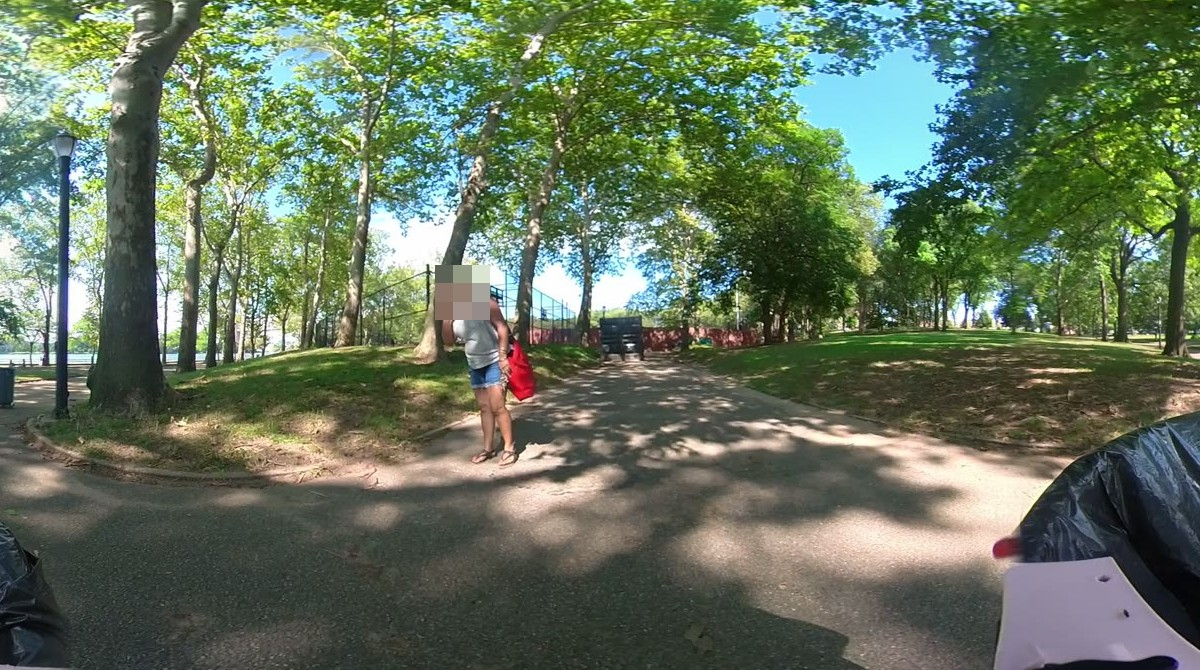
\includegraphics[width=\linewidth]{figures/vignettes/g_astoria_watch.jpg}
    \caption{14:51}
  \end{subfigure}\hfill
  \begin{subfigure}[t]{0.49\columnwidth}
    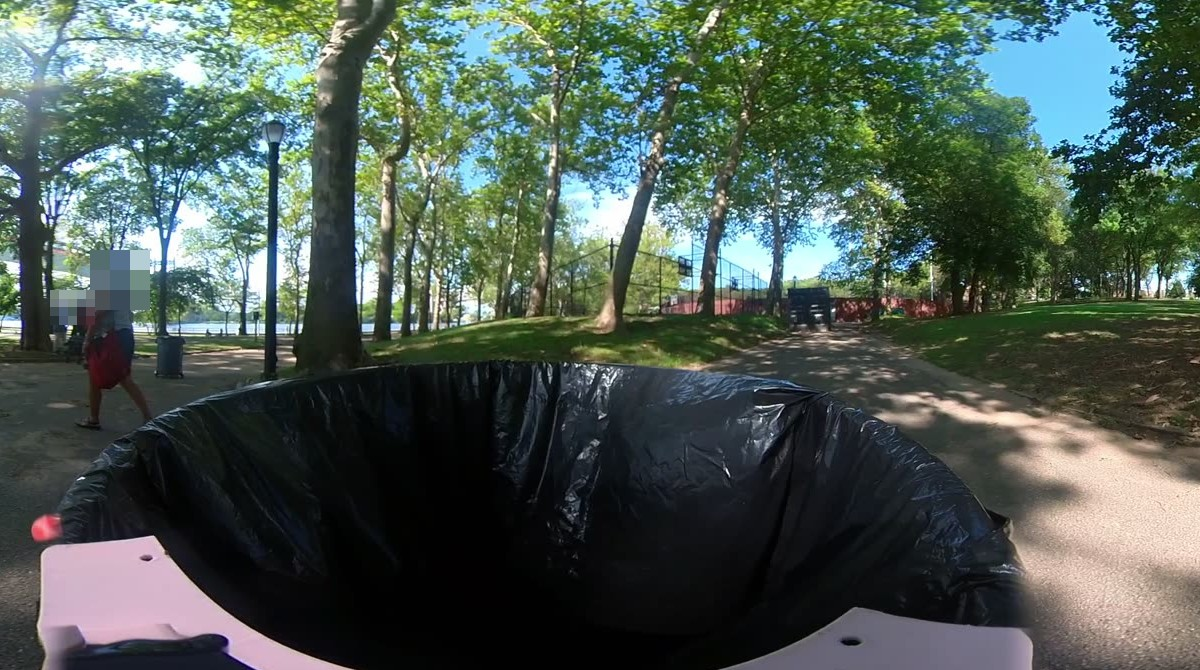
\includegraphics[width=\linewidth]{figures/vignettes/h_astoria_retreat.jpg}
    \caption{14:57}
  \end{subfigure}
  \caption{Astoria Park, 16 July, from the barrel's rim (faces obscured). The
  participant stands on the path watching the robot (a), then, as it turns
  toward her, moves off and keeps watching from farther away (b). The
  interview that followed is the measured appraisal quoted in the text.}
  \Description{Two photographs from the trash barrel robot's rim camera on a
  shaded park path. In the first a woman with a red bag stands on the path
  facing the barrel; in the second she is walking away along the path to the
  left while the barrel's black liner fills the foreground. Faces are
  pixelated.}
  \label{fig:retreat}
\end{figure}

The Astoria Park case runs the other way. On the onboard recording of 16 July a
participant watches the robot with evident curiosity, screams and moves away
each time it approaches, and keeps watching from a greater distance
(Figure~\ref{fig:retreat}). The
interview that follows is measured and analytic: the robot will be stolen or
vandalized (\pquote{I think people will just take them}), a municipal version
would read as someone watching and fail the way the police robot dogs did, a
park is a better place for it than a street where people are in a hurry, and,
weighed against all that, \pquote{at least it's kind of friendly, right? Doesn't
have any weapons}. Nothing in the account mentions the startle, and nothing in
the conduct anticipates the appraisal.

That the gap opens in both directions matters. If interviews simply added a
layer of caution or social desirability to what people had done, divergence
would run one way: use followed by disavowal. It also runs from avoidance to
appraisal. A stable-attitude account has to treat one record in each pair as
noise. A situated account does not. The disposal on Arthur Avenue was answering
the question ``is this a bin''; the interview was answering a different
question, put by a stranger with a microphone, for which sidewalk width and
winter are exactly the sort of thing a person reaches for. The retreat at
Astoria Park was answering ``what is this thing doing near me''; the interview
was answering ``what would this mean for the city,'' and that answer is
assembled from theft, surveillance and robot dogs, not from the startle.

\paragraph{Trajectory.}
Trajectory shows the assembly happening. One Little Italy participant saw the
robot and its camera from a block away and came over alarmed---\pquote{oh, what
the hell?}---was reassured by an account of the research purpose, and then, on
learning that a person was driving the machine, re-described it as a game:
\pquote{It's like playing a PS spot.} He was not given new information about
what the robot does, or what it records, or who would see the footage. He was
told that somebody was holding a controller. The question that had been open
was \emph{who runs this}, and it was answered by making the operator visible
rather than by explaining the system. We should be plain about how this
sequence became observable: telling him departed from our approved procedure,
which asked researchers not to disclose the operating arrangement during the
encounter (\S\ref{sec:limitations}). The trajectory was produced, inadvertently,
by a researcher answering the question the participant had actually asked.

The same resolution occurred at Tappen Park without any disclosure, because the
participant supplied it himself. His first reaction to the barrel was the one
\S\ref{sec:inputs} would predict for that park---\pquote{I was wondering if you
guys were recording me}---and what dissolved it was not anything we said but
something he worked out: \pquote{I was really curious to know what you guys
were doing, and then I see it move towards me, then I realized that you guys
were operating it \ldots so I wasn't scared}. Asked why the robot had come to
him, he answered \pquote{I thought you guys directed it to me}, and the
researcher's reply that it was autonomous did not dislodge the inference. He
went on to argue that without a camera the machine would be obvious, and that
with one, approaching \pquote{out of the blue}, it would frighten him. The
operator he had located was doing for him what the disclosure did for the
Little Italy participant. We have not located his encounter on the onboard
record, so this is an account of a trajectory rather than a paired case; we
include it because it shows the mechanism working unprompted. The Tappen Park
refusal, read as a sequence rather than an outcome, is a trajectory of the
opposite sign: a \emph{Star Wars} reference, then a camera that would not stop
looking, then the kick. His own summary is the cleanest statement of it:
\pquote{that's why it turned from cute to offensive}.

\paragraph{What the paired cases license.}
Read together, these cases support a specific claim and not a stronger one. We
are not saying that participants were insincere, that interviews are
unreliable, or that behavior is the truth against which talk should be checked.
We are saying that the account and the conduct were produced at different
moments, under different demands, and that the account is a situated production
in its own right---which is why it can recruit a concern the conduct never
consulted, and why it diverges from conduct in both directions. In every
trajectory we can trace, what moved the account was the standing of one
question, who is behind the machine. Answered, by disclosure or by the
participant's own inference, the unease dissolved faster than any explanation
of the system could have managed; left open while the camera kept looking, it
hardened into refusal. That is the finding the Discussion builds on. It is also
the limit of what this material can carry. Onboard coverage has been reviewed
for the Queens, Staten Island and Bronx sessions and not yet for Manhattan or
Brooklyn; the rim of the barrel is in frame for only part of each recording;
and the cases above are the ones the record supports, not a sample of
encounters. We therefore report the relationships as kinds, not as rates, and
make no comparison of their frequency between sites.
% \note{Case sources for verification before camera-ready. Astoria 15 Jul:
% \texttt{IMG\_1745} + \texttt{VID\_20250616\_054414\_00\_011} 25:38--25:44
% (frame-verified). Tappen trial: \texttt{IMG\_7447} (full NAS copy; the Box
% \texttt{TP-P11} cut is truncated) + \texttt{VID\_20250608\_051940\_00\_001}
% 00:40--01:39 (recycling barrel; found 2026-09-02 from the corpus overview
% deck's TP-P10 entry---the earlier pairing log's ``footage missing'' verdict
% was wrong, it had only checked the liner). Tappen refusal:
% \texttt{TP-P09-conduct} + \texttt{TP-P09-interview}. Arthur Avenue:
% \texttt{BX0929-I3} + \texttt{VID\_20250831\_040052\_00\_012\_360} 22:06--22:39
% (deck LI-P27); the two at the table reach across the rim at 22:34--22:35.
% \textbf{Consent status of the Arthur Avenue frames (Figure~\ref{fig:arthur}):}
% the caf\'e-table participant consented to audio only (interview 00:12--00:25);
% the public-safety officer of \texttt{BX0929-I4} declined both audio and video
% (01:12), so he is shown with his back to the camera and is not quoted; the
% cart vendor's cut (\texttt{BX0929-I5}) contains no recording request---find it
% on the DJI file around 17:00--17:25. The team's decision (2026-09-03) is to
% publish these frames de-identified (faces pixelated); clear that decision with
% the IRB record before camera-ready, since two of the three declined video.
% Astoria 16 Jul: \texttt{IMG\_1762} +
% \texttt{VID\_20250617\_071550\_00\_015} 14:44--15:13 as logged in the deck
% (AP-P06 there); the frames at 14:51--14:57 show an adult woman with a red bag
% moving off, consistent with the deck's linkage, but confirm she is the
% interviewee, and check whether the lines at 01:03 and 01:10 of the interview
% (``don't worry, robot garbage \ldots no big brother watching you'') are the
% participant reassuring a companion---if so they are worth quoting. Little
% Italy trajectory: \texttt{092925-03}. Tappen operator: \texttt{IMG\_7448}, the
% same interview as the onboard-audio cut \texttt{TP-P08-interview}; the deck
% places his encounter at \texttt{\_003} 00:30--01:44. Recording statements:
% researchers told the Tappen refusal participant (\texttt{TP-P09-interview}
% 00:19), the Astoria 15 Jul family (\texttt{IMG\_1745} 03:45) and the Astoria
% 16 Jul group (\texttt{IMG\_1762} 00:59) that the onboard camera was not
% recording video; the frames in Figures~\ref{fig:vignettes} and
% \ref{fig:retreat} come from that camera, so clear their publication against
% the IRB record of the reported departures before camera-ready.
% Figure~\ref{fig:everyday}: (a) \texttt{2025-07-01-gopro-1.mp4} 01:24 (deck
% TP-P02, interview \texttt{IMG\_7397}); (b)
% \texttt{VID\_20250618\_055026\_00\_018} 10:11 (deck AP-P08, interview
% \texttt{IMG\_1880}). All quotations
% in this subsection are from working ASR transcripts and need audio
% verification per \S\ref{sec:interview-analysis}. Earlier drafts ran divergence
% as a two-case claim built on \texttt{IMG\_1747}; that case was closed on both
% sides on 2026-08-25 and must not be restored.}

